% LaTeX Template for Project Report, Version 2.0
% (Abstracted from a Major Project Report at CSED, NIT Calicut but can be
% modified easily to use for other reports also.)
%
% Released under Creative Commons Attribution license (CC-BY)
% Info: http://creativecommons.org/licenses/by/3.0/
%
% Created by: Kartik Singhal
% BTech CSE Batch of 2009-13
% NIT Calicut
% Contact Info: kartiksinghal@gmail.com
%
% It is advisable to learn the basics of LaTeX before using this template.
% A good resource to start with is http://en.wikibooks.org/wiki/LaTeX/
%
% All template fields are marked with a pair of angular brackets e.g. <title here>
% except for the ones defining citation names in ref.tex.
%
% Empty space after chapter/section/subsection titles can be used to insert text.
%
% Just compile this file using pdflatex after making all required changes.


\documentclass[12pt,a4paper]{report}
\usepackage{tabularx}
\usepackage{float}
\usepackage[pdftex]{graphicx} %for embedding images
\usepackage{url} %for proper url entries
\usepackage[bookmarks, colorlinks=false, pdfborder={0 0 0}, pdftitle={Final Report}, pdfauthor={Dibyan Goswami}, pdfsubject={Negative Bias Temperature Instability on pMOS}, pdfkeywords={<keywords here>}]{hyperref} %for creating links in the pdf version and other additional pdf attributes, no effect on the printed document
%\usepackage[final]{pdfpages} %for embedding another pdf, remove if not required

\begin{document}
\renewcommand\bibname{References} %Renames "Bibliography" to "References" on ref page

%include other pages
\begin{titlepage}

\begin{center}

\textup{\small {\bf Final Project} \\ Report}\\[0.2in]

% Title
\Large \textbf {Study of Bias Temperature Instability in \\180 nm pMOS}\\[0.5in]

       \small \emph{Submitted in partial fulfillment of\\
        the requirements for }
        \vspace{.2in}

       \normalsize {\bf Summer Internship }\\[0.2in]

% Submitted by
\small Submitted by \\

Dibyan Goswami \\B.Tech-School of Electrical Engineering, VIT Vellore \\

\includegraphics[width=0.4\textwidth]{./vit-logo}\\[0.1in]

%\vfill
%\vspace{.1in}
Under the guidance of\\
{\textbf{Dr. Shammi Verma\\Scientist/Engineer, QARG}}\\[0.2in]



% Bottom of the page

\includegraphics[width=0.3\textwidth]{./scl-logo}\\[0.2in]
\Large{Semiconductor Laboratory}\\
\Large
\textsc{Department of Space, Government of India}\\
\normalsize{Sector 72, S.A.S Nagar, Punjab, India -- 160 071} \\
\vspace{0.2cm}
June 2022

\end{center}

\end{titlepage}

\newpage
\thispagestyle{empty}

\begin{center}

%\huge{Semiconductor Laboratory}\\[0.5cm]
%\normalsize
%\textsc{Department of Space, Government of India}\\[2.0cm]

\emph{\huge Declaration}\\[2.5cm]
\end{center}
\normalsize This is to certify that this is a bonafide record of the Summer Internship undertaken by Dibyan Goswami-20BEE0059 at Semiconductor Laboratory, Mohali during June 2022 in partial fulfilment of the requirements of the degree of Bachelor of Technology in Electrical and Electronics Engineering from VIT Vellore.\\[1.0cm]





\vfill


\vspace{2in}

\noindent\textbf{Dibyan Goswami}
\hfill
\textbf{{Dr. Shammi Verma}} \\
(Student Intern)
\hfill
(Project Mentor)


\vspace*{\fill}\begin{flushleft}
Date: 29 June 2022
\end{flushleft}

\cleardoublepage
%\pagebreak
\phantomsection

\chapter*{Acknowledgments}
\vspace{1.0in}
I would like to convey my gratitude to Dr. Surinder Singh, Director, SCL for providing me with this unique opportunity of interning in their prestigious institute.

I am thankful to Mr. Kul Bhushan, HRDD for assigning me my project work and department and conducting lab visits that helped me get a better understanding of the fabrication, packaging and testing process. 

I thank Mr. Anil Singh, Group Head, QARG  for assigning me my project topic and Dr. Chumki Saha, Head, PRQAD for assigning me to my mentor and guiding me during the course of my internship.

I would like to acknowledge with gratitude, the support and guidance provided by my mentor, Dr. Shammi Verma, Sci./Engineer, QARG during the course of my internship and providing me with a good learning experience. I am grateful to the technicians from PRQAD lab for providing technical support during the experiment. 

Finally, I would like to thank my fellow interns who made the learning process a fun experience and helped whenever it was needed. I would like to thank my parents for their support and constant encouragement. 
\\
\\
\\ 
\\
Dibyan Goswami \\ 
\\
June 2022\\
{Semiconductor Laboratory}\\
\newpage


\pagenumbering{roman} %numbering before main content starts
\tableofcontents
\listoffigures

\newpage
\pagenumbering{arabic} %reset numbering to normal for the main content

%\chapter{Problem Definition}

Negative Bias Temperature Instability is a failure mode in MOSFETs. NBTI manifests itself in the form of increase in threshold voltage and a consequent decrease of drain current and therefore transconductance of the MOSFET. NBTI is of a concern in pMOSFETs that operate under negative voltage and has been on the rise with incorporation of Nitrogen in the oxide layer and decrease in MOSFET size with every technological node. It is therefore of importance to test fabricated pMOSFETs for NBTI and understanding the test conditions and how to identify a faulty device after testing.
 %objective changed to problem definition
\chapter{Introduction to Project}

If software was a person then Silicon would be its water. Si has made the software revolution possible. Semiconductors allow us to realise boolean logics on the nanoscale and ultimately allow us to integrate several of them together to build an Integrated Circuit. ICs play an important role in control applications everywhere. There are ICs everywhere around us, from the air-conditioner cooling our room to the car taking us to office. It is therefore, of importance to us to understand semiconductors, their working and their shortcomings to become good hardware engineers who can develop high quality ICs that not just ease our lives but make scientific and technological innovations easier to achieve. In this report, we start by discussing about Silicon: its fabrication process. We then talk about CMOS fabrication and MOSFET operation. Towards the end we discuss the failure modes of a MOSFET and the short channel effects. Finally, we discuss about NBTI and NBTI testing. Negative Bias Temperature Instability is a failure mode in MOSFETs. NBTI manifests itself in the form of increase in threshold voltage and a consequent decrease of drain current and therefore transconductance of the MOSFET. NBTI is of a concern in pMOSFETs that operate under negative voltage and has been on the rise with incorporation of Nitrogen in the oxide layer and decrease in MOSFET size with every technological node. It is therefore of importance to test fabricated pMOSFETs for NBTI and understanding the test conditions and how to identify a faulty device after testing. %literature survey included in this
\chapter{Fabrication Process of CMOS}

\section{Silicon Processing}

\subsection{Why Do We Use Silicon}
We prefer Si for fabricating MOSFETs. Si is an ideal bulk semiconductor as it is easily available in large quantities, it has a bandgap of 1.12 eV which is greater than that of Germanium (0.67 eV) which means it absorbs and emits radiation in the visible region. Si can be worked at higher temperatures while Ge crystals disintegrate upon heating. Si also forms a protective SiO2 layer simply on heating which is hydrophobic in nature and eases the process of fabricating MOSFETs by acting as a barrier between bulk Si and Gate contact.



\begin{figure}[htb]
\centering

\includegraphics[scale=0.6]{./fig1} % e.g. insert ./image for image.png in the working directory, adjust scale as necessary
\caption{Silicon is widely available in nature in the form of sand}
\label{3.1} % insert suitable label, this is used to refer to a fig from within the text as shown above
\end{figure}

\subsection{Process of obtaining Silicon}
First step is simple, we reduce silica sand obtained from nature with coke to obtain Metallurgical Grade Silicon (MGS) of 98% purity.
We then treat MGS with hydrochloric acid to obtain Trichlorosilane. Impurities in MGS are converted to FeCl3, BCl3, PCl3/ PCl5 which can be removed by distillation. 
Trichlorosilane on further hydrogenation produces Si. This gives us highly pure silicon called Electronic Grade Silicon (EGS).

\subsection{Silicon Wafering }
We use the EGS obtained to produce wafers. We melt EGS in a crucible and inject a Si seed of a known orientation and rotate it and pull out the silicon melt at a slow rate. It is necessary for it to be a slow rate so that the silicon melt crystallises into the crystal of the same orientation as the seed without deformities and defects. 



\begin{figure}[htb]
\centering
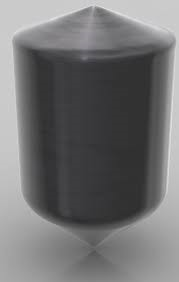
\includegraphics[scale=0.4]{./fig2} % e.g. insert ./image for image.png in the working directory, adjust scale as necessary
\caption{A Silicon ingot}
\label{3.2} % insert suitable label, this is used to refer to a fig from within the text as shown above
\end{figure}

\noindent Once the silicon ingot is obtained, we confirm crystal orientation using X-ray diffraction. We then grind a flat or notch on the ingot for the desired crystal orientation and saw it into wafers. We remove surface taper by lapping. As Si is brittle it is essential for there to be no cracks as they propagate through the entire surface. Therefore, we smoothen the edges using edge smoothening. After this we use laser scribing to ID the wafer and then etch it to remove damages caused by lapping and then polish it. Polishing allows us to thin the wafers further and remove contaminants on the surface.



\begin{figure}[htb]
\centering
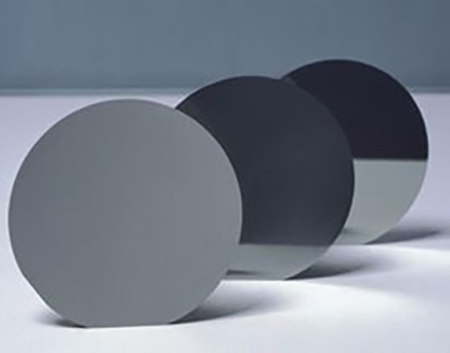
\includegraphics[scale=0.3]{./fig3} % e.g. insert ./image for image.png in the working directory, adjust scale as necessary
\caption{A Silicon wafer}
\label{fig:label} % insert suitable label, this is used to refer to a fig from within the text as shown above
\end{figure}

\pagebreak


\section{CMOS Fabrication}
In CMOS fabrication we start with a Si layer that is either p-type or n-type. Let us consider a p-type substrate in our case. 

\begin{figure}[htb]
\centering
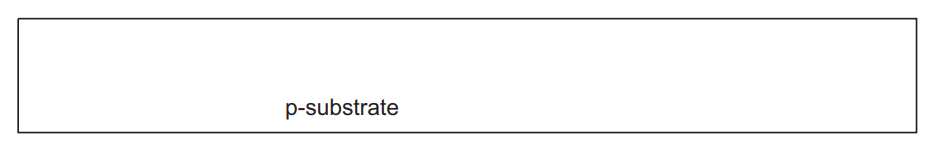
\includegraphics[scale=0.3]{./fig4} % e.g. insert ./image for image.png in the working directory, adjust scale as necessary
\caption{bare wafer}
\label{3.4} % insert suitable label, this is used to refer to a fig from within the text as shown above
\end{figure}

 
\noindent It is heated in a furnace to form a protective layer of SiO2. 

\begin{figure}[htb]
\centering
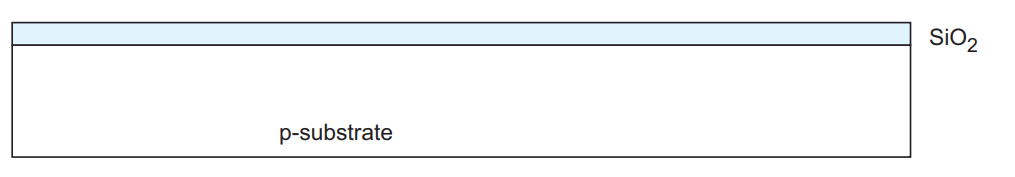
\includegraphics[scale=0.3]{./fig5} % e.g. insert ./image for image.png in the working directory, adjust scale as necessary
\caption{Oxide coating}
\label{3.5} % insert suitable label, this is used to refer to a fig from within the text as shown above
\end{figure}
 
\noindent We then add a photoresist over this layer. 

\begin{figure}[htb]
\centering
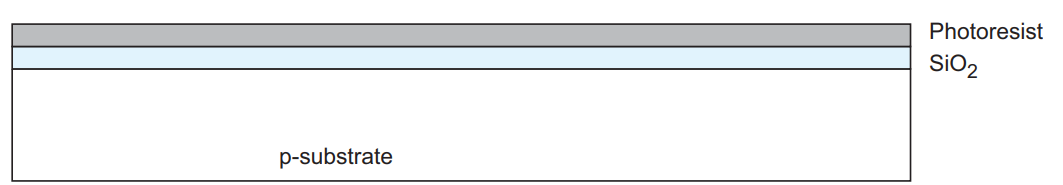
\includegraphics[scale=0.3]{./fig6} % e.g. insert ./image for image.png in the working directory, adjust scale as necessary
\caption{Photoresist coating}
\label{3.6} % insert suitable label, this is used to refer to a fig from within the text as shown above
\end{figure}
 
\noindent Say we wish to create an n-well in the bulk Si for fabricating the pMOS. We create the mask for n-well and expose the photoresist through it making it soluble in that masked area. 
\begin{figure}[H]
\centering
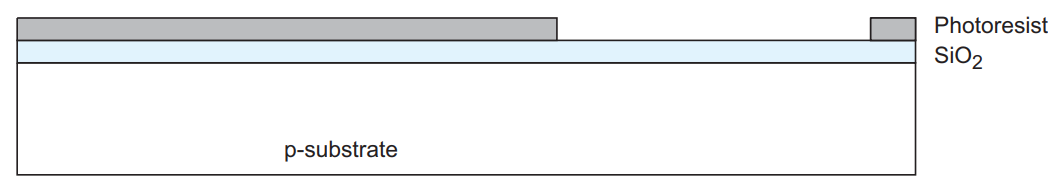
\includegraphics[scale=0.3]{./fig7} % e.g. insert ./image for image.png in the working directory, adjust scale as necessary
\caption{Masking and Etching}
\label{3.7} % insert suitable label, this is used to refer to a fig from within the text as shown above
\end{figure}
 




\noindent We etch out SiO2 layer using HF to expose the bulk Si.

\begin{figure}[H]
\centering
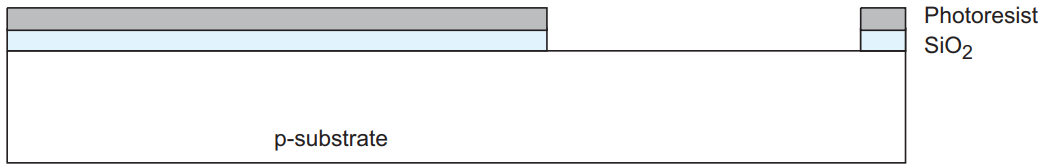
\includegraphics[scale=0.3]{./fig8} % e.g. insert ./image for image.png in the working directory, adjust scale as necessary
\caption{Oxide Etching}
\label{3.8} % insert suitable label, this is used to refer to a fig from within the text as shown above
\end{figure}
 

\noindent The remaining photoresist is removed using piranha etch.

\begin{figure}[H]
\centering
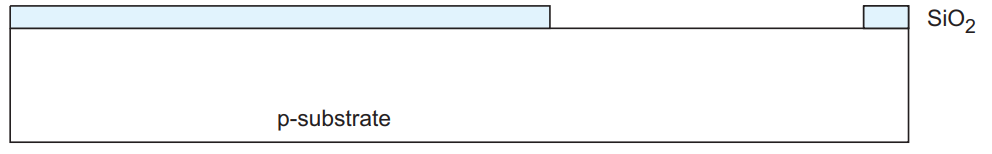
\includegraphics[scale=0.3]{./fig9} % e.g. insert ./image for image.png in the working directory, adjust scale as necessary
\caption{PR washing}
\label{3.9} % insert suitable label, this is used to refer to a fig from within the text as shown above
\end{figure}
 
\noindent We then add the n-type dopants by diffusion or ion implantation. Ion implantation provides us with the benefits of anisotropy and no lateral diffusion of dopants and better control over dopant depth.

\begin{figure}[htb]
\centering
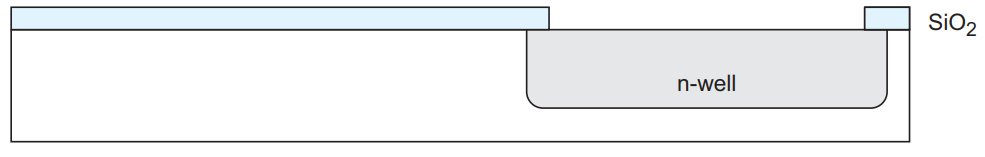
\includegraphics[scale=0.3]{./fig10} % e.g. insert ./image for image.png in the working directory, adjust scale as necessary
\caption{Ion Implantation}
\label{3.10} % insert suitable label, this is used to refer to a fig from within the text as shown above
\end{figure}
 
\noindent Excess SiO2 is removed using HF.
\begin{figure}[htb]
\centering
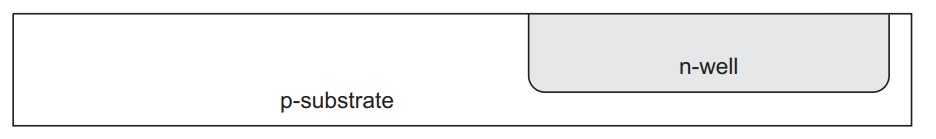
\includegraphics[scale=0.3]{./fig11} % e.g. insert ./image for image.png in the working directory, adjust scale as necessary
\caption{Etching}
\label{3.11} % insert suitable label, this is used to refer to a fig from within the text as shown above
\end{figure}
 
\noindent This gives us a Si wafer with an n-well and now we are left with generation of metal contacts and source and drain diffusion.
We once again heat the Si wafer to form SiO2. Heavily doped polysilicon is coated over SiO2 by Chemical Vapour Deposition. The wafer is heated in the presence of SiH4 to obtain wafer coated with polysilicon. 
\begin{figure}[H]
\centering
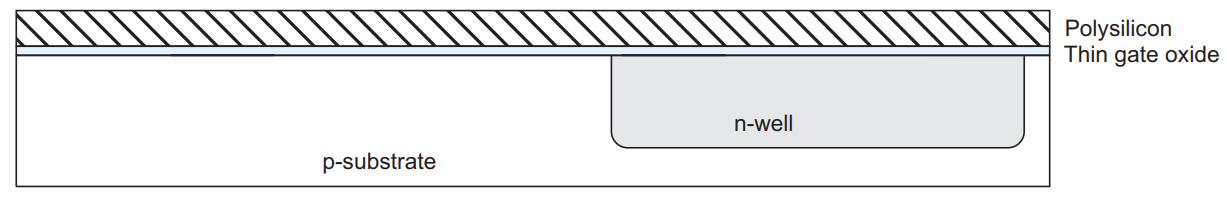
\includegraphics[scale=0.3]{./fig12} % e.g. insert ./image for image.png in the working directory, adjust scale as necessary
\caption{Polycrystalline silicon growth}
\label{3.12} % insert suitable label, this is used to refer to a fig from within the text as shown above
\end{figure}




\noindent\linebreak We pattern the area where gate contacts are to be present by using photoresist and a polysilicon mask and etch out the polysilicon and SiO2 layer from elsewhere. Leaving the gate contacts atop the oxide layer.
\begin{figure}[H]
\centering
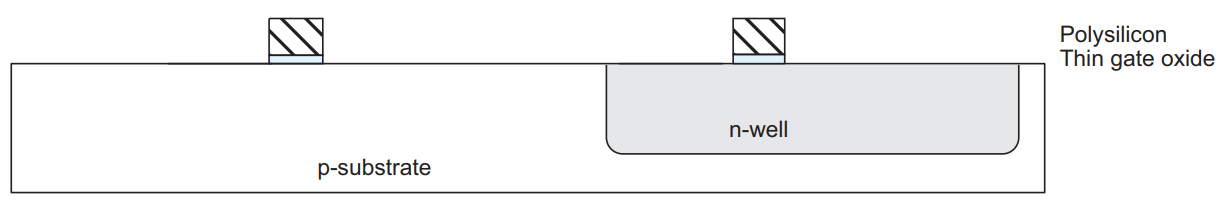
\includegraphics[scale=0.3]{./fig13} % e.g. insert ./image for image.png in the working directory, adjust scale as necessary
\caption{Gate Formation}
\label{3.13} % insert suitable label, this is used to refer to a fig from within the text as shown above
\end{figure}
 
\noindent We reheat the wafer to obtain a layer of SiO2 again and add masks in the regions where we require heavily doped n-regions for our nMOS and add dopants using the same previous method of exposure to light and etching.
\begin{figure}[H]
\centering
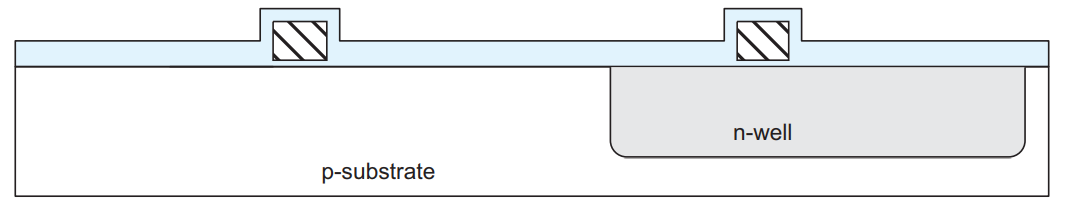
\includegraphics[scale=0.3]{./fig14} % e.g. insert ./image for image.png in the working directory, adjust scale as necessary
\caption{Oxide Growth }
\label{3.14} % insert suitable label, this is used to refer to a fig from within the text as shown above
\end{figure} 
 
\noindent We add masks to expose the region where n-type dopants are needed for the nMOS and etch out the oxide.
\begin{figure}[H]
\centering
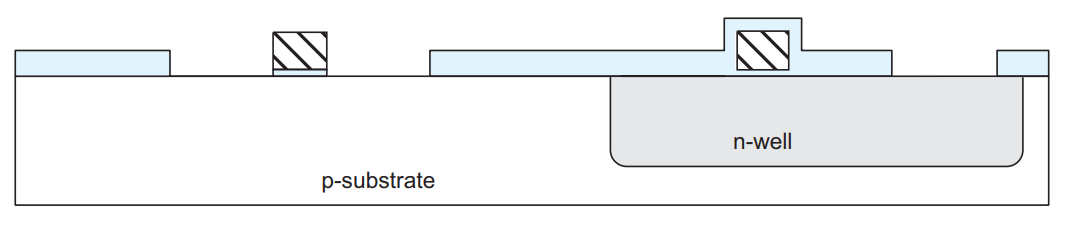
\includegraphics[scale=0.3]{./fig15} % e.g. insert ./image for image.png in the working directory, adjust scale as necessary
\caption{Source-Drain Masking and Etching}
\label{3.15} % insert suitable label, this is used to refer to a fig from within the text as shown above
\end{figure}
 
\noindent We add the n-type dopants by ion implantation. Traditionally, the dopants were diffused and therefore these regions are referred to as n-diffusion regions.
\begin{figure}[H]
\centering
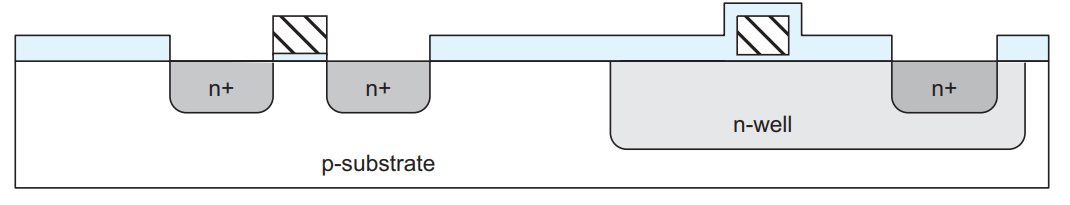
\includegraphics[scale=0.3]{./fig16} % e.g. insert ./image for image.png in the working directory, adjust scale as necessary
\caption{Dopant Implantation}
\label{3.16} % insert suitable label, this is used to refer to a fig from within the text as shown above
\end{figure}
 



\noindent We then strip off the protective oxide layer.
\begin{figure}[H]
\centering
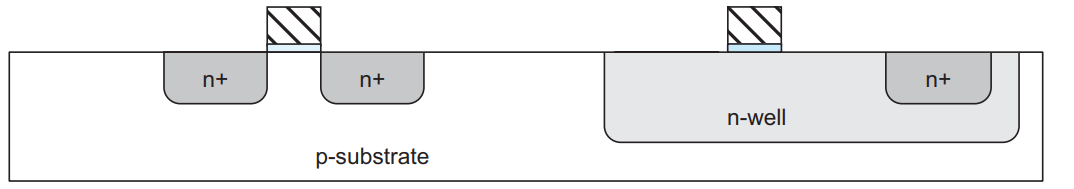
\includegraphics[scale=0.3]{./fig17} % e.g. insert ./image for image.png in the working directory, adjust scale as necessary
\caption{Oxide Etching}
\label{3.17} % insert suitable label, this is used to refer to a fig from within the text as shown above
\end{figure}
 
\noindent Similarly, we heavily dope the n-well with p type dopants to form the pMOS.
\begin{figure}[H]
\centering
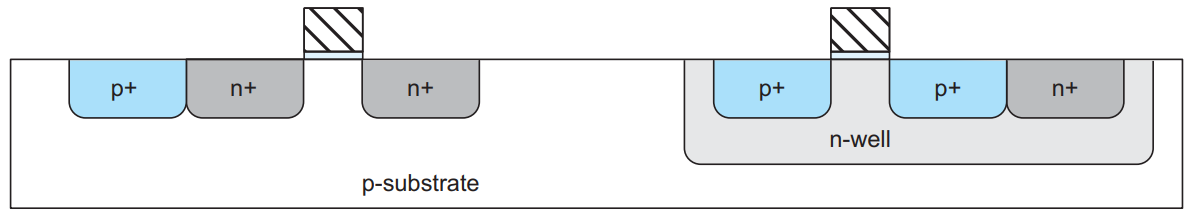
\includegraphics[scale=0.3]{./fig18} % e.g. insert ./image for image.png in the working directory, adjust scale as necessary
\caption{Fabricated CMOS}
\label{3.18} % insert suitable label, this is used to refer to a fig from within the text as shown above
\end{figure}
 
\noindent We then add masks for the metal to expose the region where metal contacts are needed.
\begin{figure}[H]
\centering
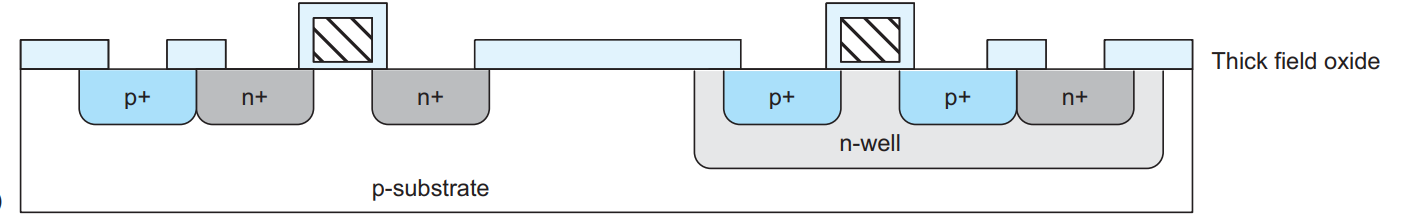
\includegraphics[scale=0.3]{./fig19} % e.g. insert ./image for image.png in the working directory, adjust scale as necessary
\caption{Fabricated CMOS}
\label{3.19} % insert suitable label, this is used to refer to a fig from within the text as shown above
\end{figure}
 
\noindent We sputter the metal over the entire wafer by blasting aluminium into vapour that evenly coats over the wafer. We use an alloy of Al and Cu. We use Cu so that Al doesn’t undergo tapering due to current flow which is a common failure mode of MOSFET called Electromigration. We remove the remaining metal from all areas by plasma etching leaving metal only where the contacts are required.
\begin{figure}[H]
\centering
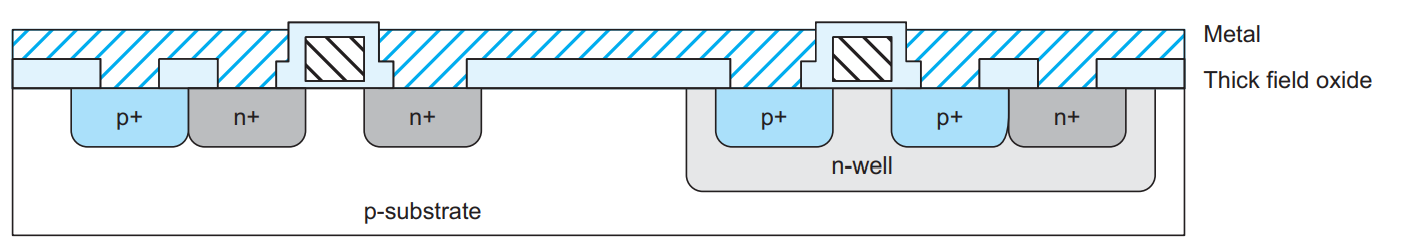
\includegraphics[scale=0.3]{./fig20} % e.g. insert ./image for image.png in the working directory, adjust scale as necessary
\caption{Fabricated CMOS with metal contacts}
\label{3.20} % insert suitable label, this is used to refer to a fig from within the text as shown above
\end{figure}








\chapter{MOSFET Operation}
MOSFET stands for Metal Oxide Semiconductor Field Effect Transistor. 
\begin{figure}[H]
\centering
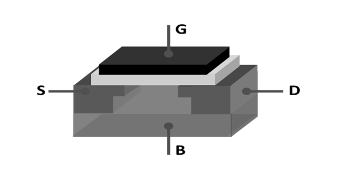
\includegraphics[scale=0.5]{./fig21} % e.g. insert ./image for image.png in the working directory, adjust scale as necessary
\caption{Simple diagram of a MOSFET}
\label{3.21} % insert suitable label, this is used to refer to a fig from within the text as shown above
\end{figure}
 
\noindent A MOSFET comprises of an Oxide layer sandwiched between a metal contact (or Polysilicon) and a semiconductor (Bulk Si). It controls current flow using an electric field applied via the Gate terminal and is therefore called a Field Effect Transistor. Carriers flow from the Source to Drain which are heavily doped semiconductors diffused into the bulk.

\section{Working of a MOSFET and IV Characteristics}
Let us consider a MOSFET with p-type bulk Si and heavily doper n-type Si at the source and drain. Initially, let gate and substrate voltage be 0 and VDD be applied to drain. As source-substrate and drain-substrate junctions are reverse biased, no current flows. We refer to this region as sub-threshold region

\begin{figure}[H]
\centering
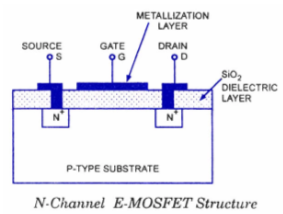
\includegraphics[scale=0.5]{./fig22} % e.g. insert ./image for image.png in the working directory, adjust scale as necessary
\caption{An N-channel enhancement mode MOSFET}
\label{3.22} % insert suitable label, this is used to refer to a fig from within the text as shown above
\end{figure}
 
 
\noindent Upon application of a gate voltage, the positive voltage attracts electrons and repels holes in the substrate. Repelled holes and incoming electrons recombine to form Si atoms. However, after a certain threshold is crossed, the accumulation of electrons overwhelms recombination. At and beyond this value of threshold gate voltage, electrons form a majority below the gate oxide and form a thin channel.

\begin{figure}[H]
\centering
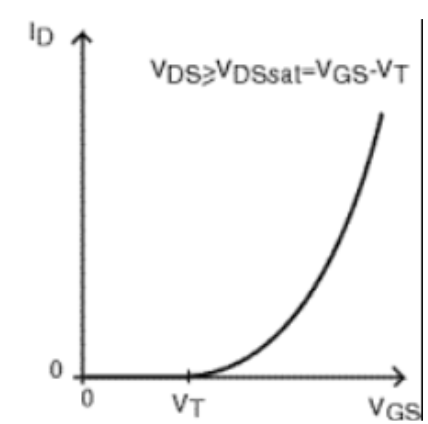
\includegraphics[scale=0.5]{./fig23} % e.g. insert ./image for image.png in the working directory, adjust scale as necessary
\caption{Drain current plotted as a function of gate voltage}
\label{3.23} % insert suitable label, this is used to refer to a fig from within the text as shown above
\end{figure}
 

\noindent As this channel is composed of electrons, it is known as an n-type channel and hence an n-type MOSFET. Also, the gate voltage enhances the concentration of n-type carriers and it is therefore an enhancement-mode MOSFET. Beyond the threshold voltage, there is a very low-resistance path for the drain current that is produced by the voltage at drain. The channel acts as a linear resistor and therefore drain current increases linearly with drain voltage. This is known as non-saturation region. 

\begin{figure}[H]
\centering
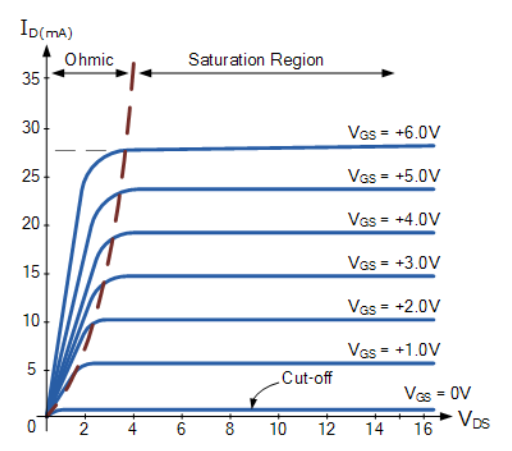
\includegraphics[scale=0.5]{./fig24} % e.g. insert ./image for image.png in the working directory, adjust scale as necessary
\caption{Drain current plotted against drain voltage}
\label{3.24} % insert suitable label, this is used to refer to a fig from within the text as shown above
\end{figure}

\noindent However, with an increase in drain voltage, the potential drop between the source and drain decreases. This reduction in potential drop across the channel lowers its width. Also, increase in drain voltage attracts n-type carriers away from the channel producing a pinch off and increasing the width of depletion region. A wider depletion region imposes greater resistance and thus drain current remains constant in spite of increasing voltage. This is known as saturation region.

\section{CV Characteristics}
\begin{figure}[H]
\centering
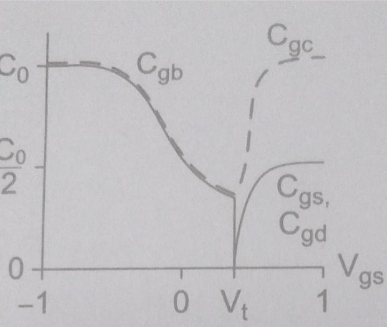
\includegraphics[scale=0.5]{./fig25} % e.g. insert ./image for image.png in the working directory, adjust scale as necessary
\caption{Capacitance plotted against gate voltage}
\label{3.25} % insert suitable label, this is used to refer to a fig from within the text as shown above
\end{figure}

Under no gate bias, the capacitance of the MOSFET equals the oxide capacitance formed between metal contact and the substrate. capacitance due to depletion regions is zero as none are formed. As gate bias is increased and channel formation begins, the effective distance between the plates increases reducing the capacitance. Upon formation of channel, for low values of drain voltage, capacitance between gate to source and gate to drain is equal hence C0/2 as they are in series.

\chapter{Reliability and Quality }
\section{Reliability Physics}
\subsection{Introduction and General Thermodynamics}
Quality refers to the property of the CMOS to work as intended without failing. Reliability is quality measured over time. Thus, reliability is a measure of the fabricated CMOS to function properly during its life. 

\noindent Our fabricated devices are prone to several failure mechanisms, for example, capacitor leakage in an IC leads to its failure. Reliability physics studies the kinetics of failure mechanisms whereas reliability engineering refers to the practices to reduce failure probability such as: proper design rules, material selection, manufacturing guidelines etc.

\begin{figure}[htb]
\centering
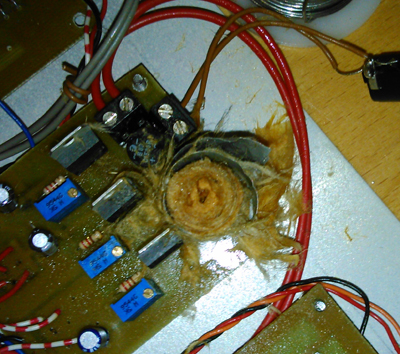
\includegraphics[scale=0.6]{./fig26} % e.g. insert ./image for image.png in the working directory, adjust scale as necessary
\caption{A capacitor that has broken down due to dielectric leakage}
\label{3.26} % insert suitable label, this is used to refer to a fig from within the text as shown above
\end{figure}

As a consequence of Moore’s law, there is a steady decrease in device size with every technology node which implies a higher current density and electric field. Thus, even during normal use a device is close to its breakdown state as the operating voltage isn’t scaled linearly with the size. Reliability studies of a device are therefore of great importance.
One might wonder, why does a device fail? In fact, most of the devices that we use are metastable i.e they are stable now but are prone to fail in the future. Devices fail because according to thermodynamics, all systems tend to assume the most stable state (possessing zero potential energy) however input energy is required to bring about this change. The Gibb’s potential is a good measure of a device’s internal energy. Let us consider a capacitor, electric field does work against conservative forces to polarize the dielectric. This increases the Gibb’s energy of the dielectric and it therefore wishes to assume a state of lower Gibb’s energy which it achieves via dielectric breakdown that lowers its internal energy to zero thus allowing it to assume a stable state.
\subsection{Hazard function}
Hazard function, h(t) is the instantaneous failure rate of a device. It tells us the number of devices that will fail, mean time-to-failure and expected number of failures in an interval. There are different types of hazard functions: constant, linearly increasing, decreasing etc, representing differing failure rates. 

For a given data, we have f(t) which is our p.d.f for failure that tells us number of failures between t and t+dt, F(t) as cumulative fraction that tells us total number of failures until t. R(t) is a measure of devices that work till time t. It is a measure of reliability. R(t)+H(t)=1 always. Hazard function is ratio of failure pdf to R(t).

\section{Reliability Statistics}
In order to determine the reliability of devices, statistics plays a crucial role as it allows us to determine a device’s lifetime, plot and visualize device data and study about their reliability, failure etc. There are three curves of importance to us; Gaussian and Lognormal distribution: used for fitting reliability data for failure due to processes like corrosion, and Weibull distribution for fitting data for weakest link failure modes.


\pagebreak
\subsection{Gaussian, Lognormal and Weibull Distribution}
Gaussian distribution is widely used for time-to-failure modelling of devices that fail due to failure modes such as corrosion. We determine the cum-fraction for each data point after arranging them in ascending order and plot Z (standard deviation) as a function of time. We get a straight-line graph with Z=0 corresponding to median (time at which 50% of the devices fail) and Z=-1 as the time at which 16% devices fail. The difference between median and the latter gives us the standard deviation. Now that we know the mean and the standard-deviation we can plot the p.d.f as a function of time to get a gaussian distribution.

\begin{figure}[htb]
\centering
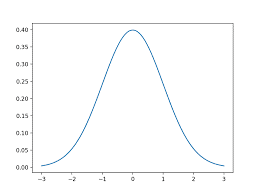
\includegraphics[scale=0.6]{./fig27} % e.g. insert ./image for image.png in the working directory, adjust scale as necessary
\caption{A gaussian distribution}
\label{3.27} % insert suitable label, this is used to refer to a fig from within the text as shown above
\end{figure}

\noindent Using the data, we can calculate instantaneous survival failure rate and average failure rate. Lognormal distribution is plotted similarly but by using a different plotting function.

\begin{figure}[htb]
\centering
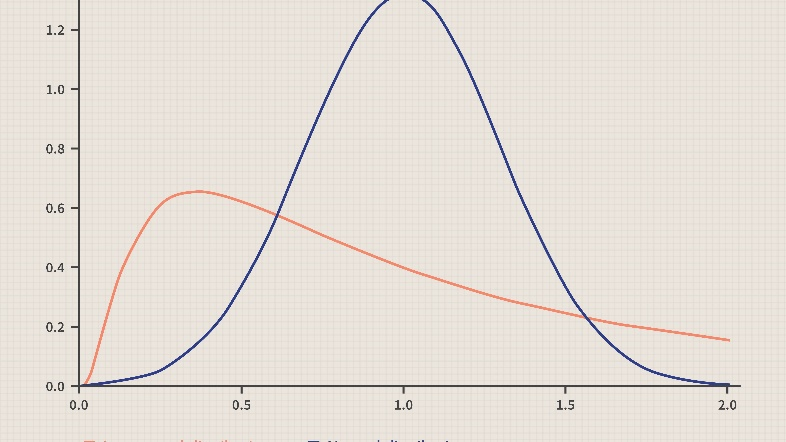
\includegraphics[scale=0.6]{./fig28} % e.g. insert ./image for image.png in the working directory, adjust scale as necessary
\caption{A lognormal distribution}
\label{3.28} % insert suitable label, this is used to refer to a fig from within the text as shown above
\end{figure}

\noindent Weibull function is used for weakest link modelling and is characterized by two parameters: time-to-failure and shape parameter. Differing values for shape parameter give us different curves allowing us to determine device stability.

\begin{figure}[H]
\centering
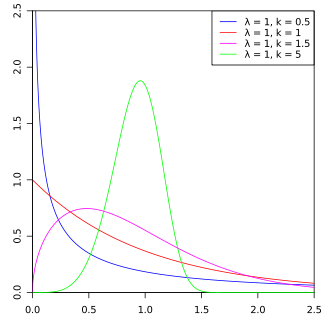
\includegraphics[scale=0.6]{./fig29} % e.g. insert ./image for image.png in the working directory, adjust scale as necessary
\caption{Weibull distribution. Differing values of shape parameter give us different graphs gaussian, exponential etc}
\label{3.28} % insert suitable label, this is used to refer to a fig from within the text as shown above
\end{figure}




\section{Bathtub Curve for Reliability }

\begin{figure}[htb]
\centering
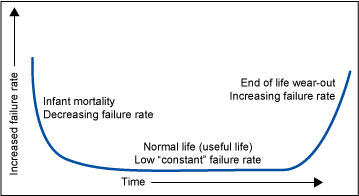
\includegraphics[scale=0.6]{./fig30} % e.g. insert ./image for image.png in the working directory, adjust scale as necessary
\caption{The bathtub curve}
\label{3.30} % insert suitable label, this is used to refer to a fig from within the text as shown above
\end{figure}


\noindent Bathtub curve is a curve that fits hazard function or failure rate as a function of time. It has three regions: EFR (Early-Failure Rate), IFR (Intrinsic-Failure Rate) and the Wear-out region. 
EFR: this region corresponds to an exponentially decreasing hazard function. This region symbolizes a very high-failure rate reducing drastically with time. In electronics, this may be due to manufacturing defects resulting in low-breakdown strength etc. 
A device can last for a year in the EFR under operating conditions. In order to remove the device from EFR region, we put it under increased stress to accelerate the time-to-failure process and this period is known as burn-in. The burn-in period is used to push the device through a year of its lifetime, if it is defective it fails during the burn-in period. The burn-in allows to remove devices from EFR and enter IFR.


\noindent IFR: this region corresponds to a low and constant hazard function. The failure rate is low and constant for a long period of time. Failure can occur in this region due to small defects.
Wear-out region: In this region, the failure rate increases monotonically with time. Failure occurs due to wear-out mechanisms resulting from long-term usage, for example, dielectric failure.
To understand the bathtub curve, we can take the example of human life. When we are born, the first year as an infant is very important and utmost care is taken. This is because infants have a very high mortality rate. Infant Mortality Rate is a concern for all societies. We take utmost care of the infant when it is born to ensure that the baby is healthy as any form of disease can be fatal. Once the baby grows up, the mortality rate is relatively very low and we don’t have to worry about our health as we did for the baby. There are few chances of us being struck by a fatal disease, we live for a long time working healthily. But as we get older, our body becomes weaker and once again we become susceptible to ailments of the old age that keep getting worse with time.
We were in the EFR as a baby, in the IFR as a boy and a man and in the Wear-out region as an old man.




\chapter{Failure Modes in MOSFETs}
\section{Failure Mechanisms}
\subsection{Time Dependent Dielectric Breakdown}
TDDB refers to the wear-out of dielectric with time. It refers to the formation of a conductive path between the gate and substrate because of which the gate field can’t control the drain current. TDDB depends on the number of defects in the gate oxide due to wafer processing, therefore to reduce it our gate oxide must be ultra-pure. TDDB occurs due to prolonged usage of the device and is not an immediate effect.  It occurs for a device in the intrinsic region of the bathtub curve

\begin{figure}[htb]
\centering
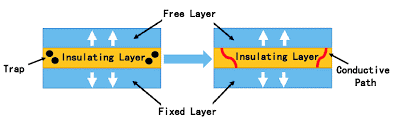
\includegraphics[scale=0.6]{./fig31} % e.g. insert ./image for image.png in the working directory, adjust scale as necessary
\caption{Traps contributing to electron tunnelling in TDDB}
\label{3.31} % insert suitable label, this is used to refer to a fig from within the text as shown above
\end{figure}


\noindent Sometimes, an electron can gain enough energy to overcome the Si-SiO2 interface potential barrier. Once this barrier is breached, electrons are accelerated through the dielectric breaking bonds thus creating traps. The traps increase the tunnelling current through the dielectric by providing a low barrier path across the dielectric to the electrons giving rise to a tunnelling current. This is a positive feedback process. The trap creation increases until the tunnelling current burns a hole in the dielectric.
\subsection{Hot Carrier Damage}
in a MOSFET, after pinch-off the lateral electrical field is restricted to the region between pinch-off and the drain contact. Thus, the electrical field increases as the length decreases increasing the drift current of the electron. This gives rise to hot electrons that may cause impact ionization, HCI, substrate leakage current and trap generation. 
\subsection{Electromigration}
EM refers to the diffusion of metal ions along the direction of electron flow in a conductor. As electrons collide with an aluminium atom, the momentum transfer increases the probability of the atom moving parallel to the electron. As the aluminium atom vacates its initial position, it creates a vacancy and instead diffuses across the conductor to fill a vacancy due to a crystal defect. When the vacancies at the initial position of the aluminium atom are not replenished, it creates a defect there. The defects coalesce to produce a large void that eventually depletes the region of all aluminium atoms in the wire leading to circuit failure.

\section{Short Channel Effects}
Short-Channel Effects refer to the effects that arise in a MOSFET when the channel length is comparable to the size of the source and drain depletion region.
 
\begin{figure}[htb]
\centering
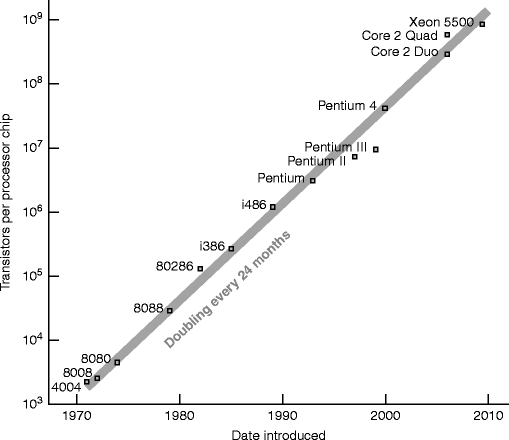
\includegraphics[scale=0.6]{./fig32} % e.g. insert ./image for image.png in the working directory, adjust scale as necessary
\caption{Graph depicting Moore’s law. Transistors per chip v. date
Short-channel effects are inevitable as a consequence of Moore’s law}
\label{3.32} % insert suitable label, this is used to refer to a fig from within the text as shown above
\end{figure}

\subsection{Drain Induced Barrier Lowering}
DIBL refers to the lowering of threshold voltage due to high drain voltage. A high drain voltage reduces the barrier voltage at the source by increasing the forward bias effect allowing easy injection of electrons from the source into the channel. Thus, the drain voltage is inducing a lowering in barrier at the source. A higher drain voltage also reduces the charges the gate voltage must balance by assuming a greater share of it. 
\subsection{Velocity Saturation}
in short channel devices, electric field is usually very high as voltage isn’t scaled linearly with channel length. Drift velocity of an electron increases linearly with electric field. Beyond a certain value of electric field, the drift velocity saturates. An electron in a short-channel device is under high electric field stress. Thus, electrons attain their saturation drift velocity much before the drain saturation voltage. At saturation velocity, the drain current also saturates and therefore current saturation occurs. But current saturation occurs before drain saturation voltage indicating that current saturation occurs as a result of drift velocity saturation and not pinch-off. This reduces the reliability of the device as it no longer saturates at a known value of drain voltage.
\subsection{Quantum Confinement}
At very small device sizes, the device size and de-broglie wavelength of electron become comparable. This implies that laws of classical mechanics no longer apply to the electron and we must use quantum mechanics to determine their behaviour.
\subsection{Hot Carrier Injection}
a hot carrier is a highly energetic charge carrier. Hot carriers are generated by incidence of photons on the substrate that creates a hole and a highly energetic electron called a hot electron. In hot carrier injection, an electron is injected from the n-channel to the gate oxide dielectric increasing its threshold voltage by oxide charging resulting in poor gate control. Holes travel out of the channel via the substrate giving rise to leakage current that can be measured to determine the extent of HCI. Hot electrons also strike the Si-H bonds at the interface generating traps that contribute to further dielectric degradation. HCI is more pronounced at low temperatures as collision probability is greatly reduced at higher temperatures due to increased vibration.
\subsection{Impact Ionization}
hot electrons can collide with other Si atoms generating electron-hole pair and increasing the drain current past saturation. 
\subsection{Mobility Degradation}
as we scale down, vertical electric field increases causing electron scattering at the Si-SiO2 interface reducing mobility of carriers.
\section{NBTI Mechanism}
NBTI is an effect that shifts the threshold voltage for a pMOS when a negative gate bias voltage is applied at elevated temperatures. NBTI arises due to trapped charges at the interface and the oxide layer. The resulting threshold voltage rise leads to a decrease in drain saturation current. The threshold voltage shift increases with stress time and reduces as the stress is removed. This is because threshold voltage shift occurs due to interface and bulk trap charges, as the negative electric field is removed, the charges diffuse back to their initial positions restoring the broken bonds and reducing the threshold voltage shift.
NBTI is more pronounced in (110) crystal lattices that have higher hole mobility due to greater density of Si-H bonds. Addition of Nitrogen induces additional hole traps in the bulk oxide. Thinner oxide layer too contributes to a greater electric field that ultimately leads to a more pronounced NBTI effect. Deuterium and Fluorine help reduce NBTI by replace the Si-H bond with a much stronger bond resulting in lesser trap generation. NBTI can be modelled by the reaction-diffusion and two-stage model. RD model describes the breaking of Si-H interface bonds by holes as a two-way process. Channel holes break the bonds that releases hydrogen that can diffuse through the oxide layer generating a hole trap. The diffusing hydrogen can also get trapped in process-induced bulk traps in the oxide layer. Electron and hole assisted tunnelling can further activate pre-existing traps. Activation of these traps ultimately rises the threshold voltage, degrading the oxide and disrupting operation.


\chapter{NBTI testing}



\section{Pre-test}
As NBTI is a prominent failure mode in 180 nm process, it is necessary for us to test our devices for failure under NBTI stress before sending them for further application. The first step in NBTI testing of a pMOS is determination of its threshold voltage. As NBTI leads to an increase in threshold voltage, we must know its nominal threshold voltage. We determine the threshold voltage of the pMOS by low-voltage of high-voltage testing. 

\noindent After determining threshold voltage, we test the device under NBTI test. For this, we use a machine integrated with a software to ease the testing process. We insert all the packages on a DUT board that has pin-outs that are connected to external circuitry in the machine. A DUT board can host several devices allowing for statistical data to be acquired.

Before NBTI, we check if gate current and drain saturation current is within an acceptable limit by applying operating gate voltage to both gate and source. We also measure the off current of the MOSFET by applying zero gate voltage.

\section{Test Conditions}
We put the device under NBTI stress by applying a temperature of 150 C and a gate voltage around 10 percent above the operating gate voltage for a period of 168 hours. The drain and source voltage must be 0. This is know as symmetrical configuration. If the device shows a deviation of 10 percent from it's initially measured threshold voltage, it is considered failed. 

While testing, we have to wait for a while before we actually make measurements after applying the stress and this period is referred to as stress soak time. This is necessary to ensure uniform application of stress conditions on the device.

\pagebreak
\section{Test Results}



\begin{tabularx}{0.8\textwidth} { 
  | >{\raggedright\arraybackslash}X 
  | >{\centering\arraybackslash}X 
  | >{\raggedleft\arraybackslash}X | }
 \hline
 Device ID & threshold voltage & leakage current \\
 \hline
 %item 21  & item 22  & item 23  \\
\hline
\end{tabularx}





\chapter{Conclusion}

The lot of pMOSFET was tested successfully under NBTI test and all the devices passed the test. The variation in threshold voltage was lesser than 10 percent indicatinmg that our devices are suitable for further use. The experiment yielded acceptable and expected values of threshold voltage and leakage current.




%\cleardoublepage
%\pagebreak
\phantomsection

\chapter*{Acknowledgments}
\vspace{1.0in}
I would like to convey my gratitude to Dr. Surinder Singh, Director, SCL for providing me with this unique opportunity of interning in their prestigious institute.

I am thankful to Mr. Kul Bhushan, HRDD for assigning me my project work and department and conducting lab visits that helped me get a better understanding of the fabrication, packaging and testing process. 

I thank Mr. Anil Singh, Group Head, QARG  for assigning me my project topic and Dr. Chumki Saha, Head, PRQAD for assigning me to my mentor and guiding me during the course of my internship.

I would like to acknowledge with gratitude, the support and guidance provided by my mentor, Dr. Shammi Verma, Sci./Engineer, QARG during the course of my internship and providing me with a good learning experience. I am grateful to the technicians from PRQAD lab for providing technical support during the experiment. 

Finally, I would like to thank my fellow interns who made the learning process a fun experience and helped whenever it was needed. I would like to thank my parents for their support and constant encouragement. 
\\
\\
\\ 
\\
Dibyan Goswami \\ 
\\
June 2022\\
{Semiconductor Laboratory}\\
\newpage

\cleardoublepage
%\pagebreak
\phantomsection
\addcontentsline{toc}{chapter}{References}
\begin{thebibliography}{99}

\bibitem{citation-1-name-here}Introduction to Microfabrication, Second Edition,\ \url{https://onlinelibrary.wiley.com/doi/book/10.1002/9781119990413}

\bibitem{citation-2-name-here}Physics of Semiconductor Devices\ \url{https://onlinelibrary.wiley.com/doi/book/10.1002/0470068329}

\bibitem{citation-3-name-here}CMOS VLSI Design: A Circuits and Systems Perspective\ \url{https://dl.acm.org/doi/10.5555/1841628}

\bibitem{citation-4-name-here}Short-Channel Effects\ \url{https://en.wikipedia.org/wiki/Short_Channel_Effects}

\bibitem{citation-5-name-here}Reliability Physics and Engineering\ \url{https://link.springer.com/book/10.1007/978-3-319-93683-3}

\bibitem{citation-6-name-here}Reliability Wearout Mechanisms in Advanced CMOS Technologies\ \url{https://ieeexplore.ieee.org/book/5361029}







\end{thebibliography}


\end{document}
